\documentclass[12pt]{report}

\usepackage{amsmath,amssymb,amsfonts}
\usepackage{listings}
\usepackage{graphicx}
\usepackage{hyperref}
\usepackage{fancyhdr}
\usepackage{color}
\usepackage{lettrine}
\usepackage{textcomp}
\usepackage[utf8]{inputenc}
\usepackage[toc,page]{appendix}
\usepackage{courier}

\usepackage[margin=2cm]{geometry}

\definecolor{dgrey}{rgb}{0.3,0.3,0.3}
\definecolor{dyellow}{rgb}{0.6,0.6,0.0}
\definecolor{gblue}{rgb}{0.35,0.35,0.6}

\hypersetup{
	colorlinks=true,
	linktoc=all,
	linkcolor=gblue,
	citecolor=dyellow,
}

\lstset{basicstyle=\ttfamily\footnotesize, frame=single,
breaklines=true,showstringspaces=false,numbers=left}

\title{ECSE 323 - Digital System Design\\After Action Report - Lab 3}
\author{Harley Wiltzer (260690006)\\Spiros-Daniel Mavroidakos(260689391)}
\date{February 23, 2017}

\begin{document}
\pagenumbering{gobble}
\maketitle
\newpage
\pagestyle{fancy}
\fancyhf{}
\rhead{Harley Wiltzer (260690006), Spiros-Daniel Mavroidakos (260689391) - Vandelay Industries}
\pagenumbering{arabic}
\tableofcontents

\part[A Modest Overture]{A Modest Overture\\\begin{center}\textnormal{\normalsize \\\textit{``My
		son, ask for thyself another kingdom; for that which I leave is too small for
	thee.''\\ - Iron Maiden - Alexander the Great, Somewhere In Time(1986)}}\end{center}}
\lettrine{S}{ince} the dawn of time, mankind has sought to make things smaller. Not so long ago, an
average computer would take up an entire room, and yet by the early 2000's Ultrium tapes were
capable of storing 100GB of data in a cartridge the size of a deck of cards. Some computers
today, such as the Raspberry Pi, are approximately the same size as a credit card. In fact,
scientist are now even capable of genetically modifying pigs to make them smaller.\\\\
The gorgeous part of this past laboratory experiment is that a complex machine was created using
hardware alone. The design was carried out without the use of any software. No sticky, hot, messy
software; no software at all. What a beautiful idea! Of course, the evident consequence of this is
that the system was created with very little overhead, and operates very quickly.\\\\
To illustrate this, consider the micro-pig.
\begin{figure}[h]
	\begin{center}
		\caption{Genetically-modified miniature pig \cite{pig}}
		\fbox{
\includegraphics[scale=0.5]{piggy1}}
	\end{center}
\end{figure}
These pigs exhibit the exact same properties as their regular-pig counterparts, but they were
genetically modified to be smaller. They are all the pig one can ask for, but in a smaller
package. Engineers designed these pigs with similar ideas to those that designed the Raspberry Pi,
and this is not surprising: if something can be designed to be smaller without sacrificing
performance, it will be done for the mere convenience of it.\\
This phenomenon is what was exhibited, more than anything, in this laboratory experiment. Fifty
years ago, had two individuals desired to play a simple game of cards, they would have to use a deck
of cards. The designs that were developed over the past two weeks will eventually allow two individuals
to play a game of cards using an FPGA that is smaller than a deck of cards.\\\\
Of course, such a feat was only possible due to the magic offered by Altera's Quartus II and
Modelsim software. Without it, the schematics and VHDL code that make up the design of this system
would never make it from the computer to the FPGA.\\\\
The process of designing what will effectively be the card deck for a digital crazy-eights game will
be documented thoroughly in the following pages of this report. Details concerning the testing of
the system will be provided, and insight concerning the design tactics will be given. Please enjoy
reading the remainder of this \textit{exposé} as much as the authors did writing it.

\part{The \texttt{g07\_stack} Circuit}
\chapter*{Introduction}
\addcontentsline{toc}{chapter}{Introduction}
The majority of this report will be concerning the design of the \texttt{g07\_stack} circuit. Note
that the \texttt{g07\_stack52} circuit is merely a circuit composed solely of the
\texttt{g07\_stack} block, which was used as a convenience for testing and integration purposes.\\\\
The goal of the \texttt{g07\_stack} circuit was to implement a stack-like data structure for the
Cyclone II FPGA. This structure will later be used to store a deck of cards for a crazy-eights game.
A stack is a canonical data structure used in computing for dynamic memory allocation. A traditional
stack follows a last-in, first-out paradigm, meaning data is added to the \textit{top} of the
structure and also
removed at the top. However, such a paradigm is not flexible enough for the purposes of the
\texttt{g07\_stack}. Not only should this circuit be capable of pushing data to the top of the stack
and \textit{popping} data back off, but it should also be able to access and remove data from an
arbitrary location
within the structure. However, according to D.A. Lowther, author of ``Computer Engineering'', ``data can only
be retrieved from the top of a stack''\cite{lowther}. \\\\
Therefore, it is clear that the use of ``stack'' in the
context of the \texttt{g07\_stack} is a misnomer. Rather, the \texttt{g07\_stack} is more akin to a
Bi-directional Jenga\textsuperscript{\textregistered} Tower (BJT), which allows objects to be pushed
to the top safely,
and can ideally have objects removed from within without causing pandemonium. Unfortunately, due to
constraints on the project, the \texttt{g07\_stack} must keep its current name. However, it is
recommended that the reader think of the \texttt{g07\_stack} as a BJT rather than a stack for its
functionality to make more intuitive sense.

\chapter*{Circuit Description}
\addcontentsline{toc}{chapter}{Circuit Description}
\begin{figure}[h]
	\begin{center}
		\caption{Pin-out diagram of \texttt{g07\_stack} circuit}
		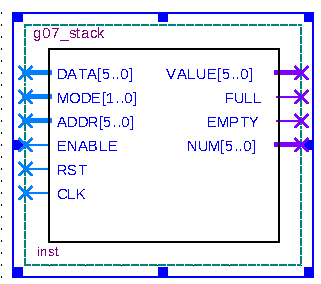
\includegraphics[scale=0.9]{Lab3/stack_symb}
	\end{center}
\end{figure}
Above is the pin-out diagram corresponding to the \texttt{g07\_stack} circuit. The input and output
ports are described below.
\section*{DATA[5..0]}
The \texttt{DATA[5..0]} port takes in a 6-bit bus which describes data that should be pushed to the
BJT when a push operation is specified.
\section*{MODE[1..0]}
The \texttt{MODE[1..0]} port takes in a 2-bit bus which represents the operation that is to be done
on the BJT. Below are the configurations of \texttt{MODE} and their meanings:
\begin{itemize}
	\item 00: NOP - No operation is done
	\item 01: PUSH - The value stored in \texttt{DATA} is pushed to the top of the structure (if it
		isn't already full). The
		value output at \texttt{NUM} is updated accordingly.
	\item 10: INIT - Values 0-51 are stored in the structure such that the top memory cell stores 0
		and the bottom one stores 51. The value at \texttt{NUM} is set to 52, and \texttt{FULL} is
		set to high.
	\item 11: POP - The value stored in the cell determined by the \texttt{ADDR} port is removed
		from the stack(if it isn't empty), and data below this address are shifted upward to remove
		the gap. The value output at \texttt{NUM} is updated accordingly.
\end{itemize}
\section*{ADDR[5..0]}
The \texttt{ADDR} port is a 6-bit bus that stores the address of the memory cell to be popped or
displayed.
\section*{ENABLE}
The \texttt{ENABLE} bit controls when the structure is enabled. When \texttt{ENABLE} is low, the
structure remains unaffected by the other inputs.
\section*{RST}
The \texttt{RST} bit, when high, asynchronously resets all memory blocks to store 0, and thus resets
\texttt{NUM} to 0, and sets \texttt{EMPTY} high.
\section*{VALUE[5..0] - Output}
The \texttt{VALUE} output port outputs the value of the data stored in the memory cell designated by
the \texttt{ADDR} input.
\section*{FULL - Output}
The \texttt{FULL} output port is set high when the value of \texttt{NUM} is 52, and low otherwise.
\section*{EMPTY - Output}
The \texttt{EMPTY} output port is set high when the value of \texttt{NUM} is 0, and low otherwise.
\section*{NUM[5..0] - Output}
The \texttt{NUM} output bus outputs a 6-bit vector representing the amount of cells being used by
the BJT. Initially, when empty, the \texttt{NUM} outputs 0. When data is pushed, \texttt{NUM}
increments, and when data is poppsed, \texttt{NUM} decrements.

\chapter*{Gate-Level Schematic}
\addcontentsline{toc}{chapter}{Gate-Level Schematic}
Due to the sheer size of the \texttt{g07\_stack} circuit, it is much more convenient to show the
gate-level schematic broken down into multiple parts. Each part will be described individually.
\section*{Enable Section}
\begin{figure}[h]
	\begin{center}
		\caption{Enable section of the circuit - controls the enable bits of the individual flip
		flops.}
		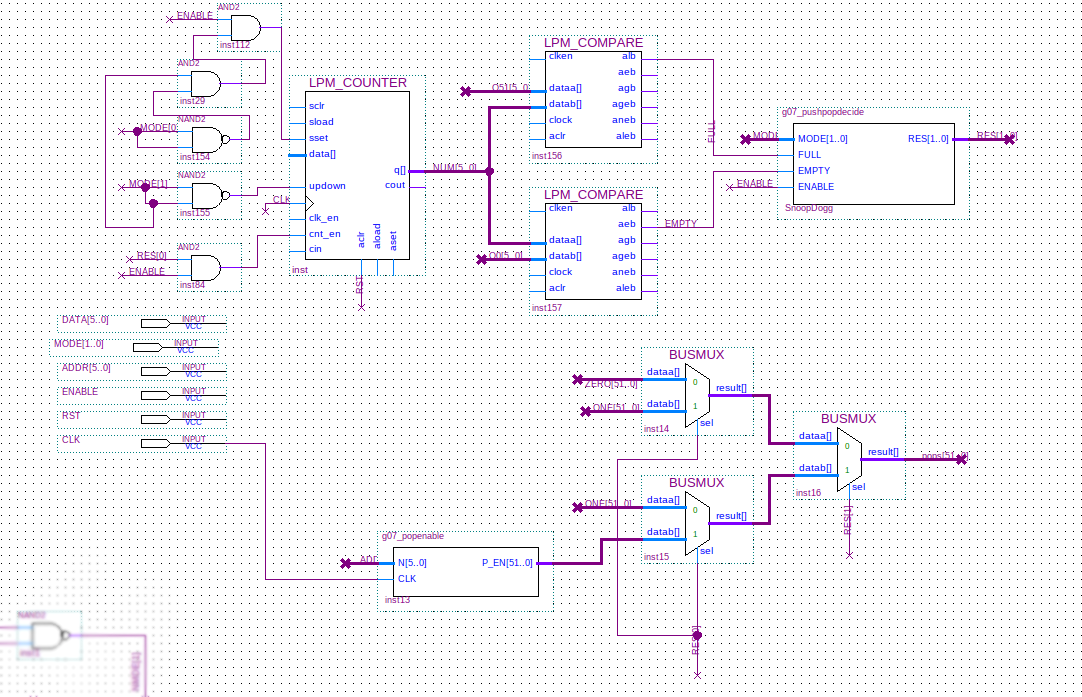
\includegraphics[scale=0.5]{stack1}
	\end{center}
\end{figure}
The enable section of the \texttt{g07\_stack} circuit is responsible for managing the enable bits on
the individual flip flops in the memory array. Flip flops must be enabled for their data to change,
however, depending on the operation requested, the flip flops that modify data may change. The upper
half of this section includes the counter used to specify the \texttt{NUM, FULL, EMPTY} outputs.
These outputs, as well as the \texttt{ENABLE, MODE} inputs are passed to the
\texttt{g07\_pushpopdecide} circuit, which sends a modified \texttt{MODE} signal called \texttt{RES}
to the lower circuit. The \texttt{g07\_pushpopdecide} circuit transforms a push instruction to a NOP
if the BJT is full, and transforms a POP instruction to a NOP if the BJT is empty. Next, the
\texttt{RES} signal is passed through a 4-1 multiplexer to choose the array of enable bits to send.
When PUSH or init are specified, the MUX outputs an array of 1's, one NOP is specified the MUX
outputs an array of 0's, and when POP is specified the MUX relays the output of the pop-enable ROM
that was designed several weeks ago. The output bits of the MUX are then passed to the memory array
via the \texttt{pops} signal.
\section*{Memory Array Section (Top)}
\begin{figure}[h]
	\begin{center}
		\caption{Top of the memory array section of the circuit - manages data to be stored in the
		BJT}
		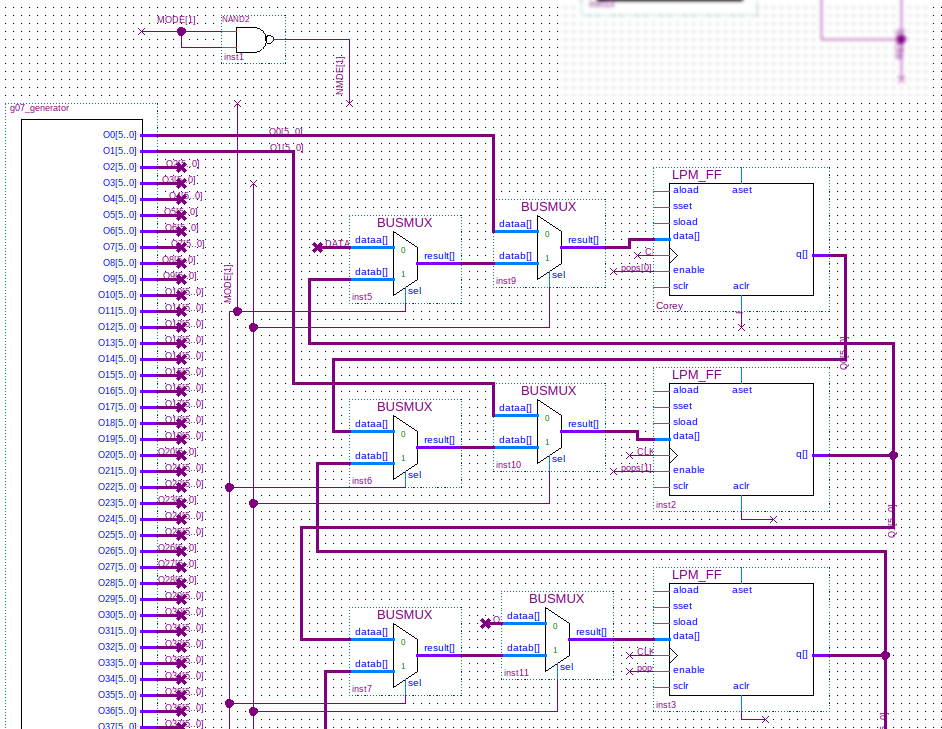
\includegraphics[scale=0.55]{Lab3/stack_array1}
	\end{center}
\end{figure}
The above diagram shows the top of the memory array. At the left end of the diagram is the
\texttt{g07\_generator} subcircuit, which was designed to store the constants 0-51 as 6-bit vectors.
For convenience, a 52-bit array of 1's and a 52-bit array of 0's was also included. This circuit was
designed with VHDL code that was generated with Haskell code, which can be perused 
\hyperref[app:hs]{here}.
Between the \texttt{g07\_generator} and the flip flops lie two columns of MUX's. Each flip flop is
associated to two MUX's which choose which data to pass to its \texttt{data} input. The leftmost
MUX's take in the data from the flip flop above it and the data from the flip flop below it, so as
to accomodate data shifting in both directions (which is why it's called a \textit{bidirectional}
Jenga\textsuperscript{\textregistered} tower). This MUX takes the most-significant bit of the
\texttt{MODE} input as its select line. Then, the rightmost MUX takes in the output of the leftmost
MUX and the corresponding constant from the \texttt{g07\_generator} as its data inputs, and takes
the least-significant bit of the \texttt{MODE} signal as its select line. This MUX chooses whether
to load data from another memory cell (push or pop) or load a constant (init) to its corresponding
flip flop.\\\\
The BJT continues on in this fashion all the way to the bottom, and is not shown in its entirety
since no additional logic is available. However, the bottom portion of the BJT will be displayed,
which shows some extra circuitry.

\section*{Memory Array Section (Bottom)}
\begin{figure}[h]
	\begin{center}
		\caption{Bottom of the memory array section of the circuit - manages data to be stored in the
			BJT, manages the \texttt{VALUE} output.}
		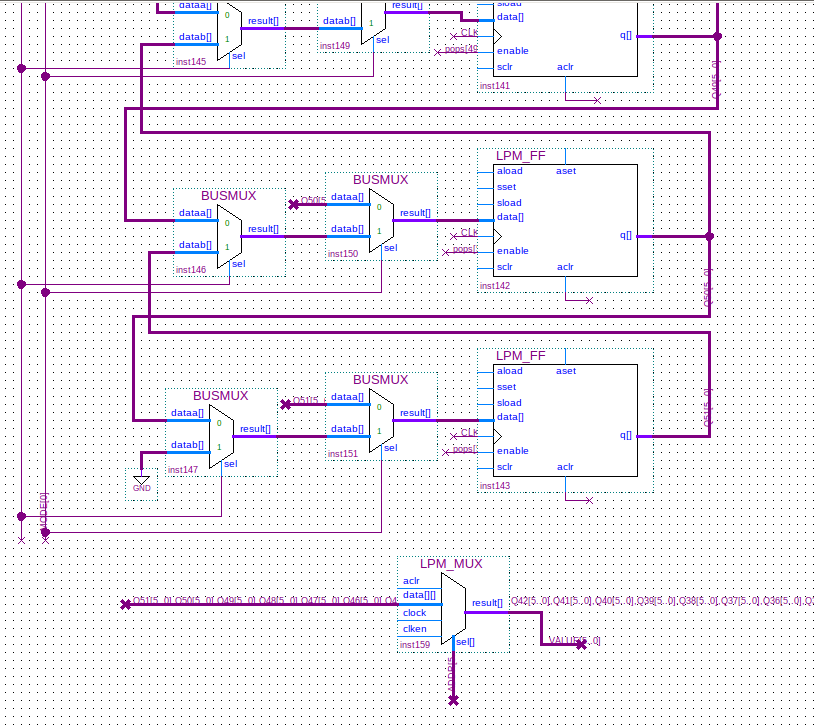
\includegraphics[scale=0.6]{Lab3/stack_array2}
	\end{center}
\end{figure}
Here, the last three memory cells of the BJT are displayed. Note that the bottom memory cell has a
grounded input at its leftmost MUX, which effectively loads 0 to the bottom element when a pop
operation is carried out. Finally, below the bottom memory cell lies the logic that manages the
\texttt{VALUE} output. It takes the form of another MUX, which takes every flip flop value as data
inputs, and uses the \texttt{ADDR} input as its select line.
\part{On the Testing of the \texttt{g07\_stack} Circuit}
\chapter*{Overview}
\addcontentsline{toc}{chapter}{Overview}
Naturally, with a circuit as complex as the \texttt{g07\_stack}, it is imperative that testing is
done thoroughly. Of course, the \texttt{g07\_stack} supports four commands, which, when considering
branches in logic depending on the current state of the BJT, may support an unwieldly amount of
input combinations. Thus, in the effort to test the \texttt{g07\_stack} circuit, the goal was simply
to test each functionality and its edge cases rather than each possible input scenario.\\
To do this, the \texttt{g07\_testbed} was created. This circuit is composed of the
\texttt{g07\_stack}, as well as the simple \texttt{mod13} circuit and some
\texttt{g07\_7\_segment\_decoder} circuits. The testbed was created so that the \texttt{g07\_stack}
could be tested on the Altera DE1 board and produce visual, comprehensive output. Please consult
\hyperref[app:testbedvhdl]{this appendix} for the testbed's VHDL code.\\\\
However, the elements that have been described are not good enough on their own for the practical
testing of the \texttt{g07\_stack} on the DE1 board, as they do not account for the all-feared
button bounce problem. For the interested reader, a description of this problem and how it was
solved is included in the interlude below.
\section*{The \texttt{g07\_debounder} Circuit: A Brief Interlude}
\addcontentsline{toc}{section}{The \texttt{g07\_debounder} Circuit: A Brief Interlude}
When dealing with physical buttons, all hell may very well break loose. Unless the button is ideal
(and it isn't), pressing the button once will not actually look like one button press to the
electronics that the button is connected to.\\\\
This is what is known as the button bouncing problem, and it must be solved immediately to carry out
the desired tests. It was decided that a \textit{debouncing circuit} should be created, which led to
the conception of the \texttt{g07\_debounder}\footnote{Notice the simple typo in the name of the
	\texttt{g07\_debounder}. This typo was committed by Harley Wiltzer when rushing through the
	design of the circuit, which was done during a time when he had ``other work to do''. Later on,
	when the success of the circuit put Wiltzer and Mavroidakos in a state of enlightenment, they
realized that the typo was present. However, they left the typo there for sentimental purposes.}.
The purpose of this circuit was to remove the
``bouncing'' of the button output. But what \textit{is} bouncing? Is bouncing the process of moving
along in a lively manner while repeatedly striking the surface below and rebounding? Or is bouncing
the act of removing a vicious intoxicated person from Sir Winston Churchill's? For the sake of the
\texttt{g07\_debounder} circuit, bouncing will be modeled as a phenomenon similar to the former.\\\\
Button presses tend to cause the inner metal contacts to \textit{bounce}, which causes the circuit
to open and close repetitively in an unpredictable manner. Therefore, without the
\texttt{g07\_debounder} circuit, each button press would actually cause multiple pulses to be sent
to the \texttt{g07\_stack}, which is a severe issue. The \texttt{g07\_debounder} circuit was
designed to only register one clock pulse of high output within a $2^{23}$ clock-pulse period. This
sets a limit on how frequently button presses can be registered, but it also removes the possibility
of registering multiple pulses from one button press.\\\\
To achieve this functionality, a Moore-type finite state machine was designed. This machine includes
two SR Flip Flops to store the current state of the machine, as well as a 23-bit counter to count
clock pulses since the button was first pressed. The counter output is fed to a comparator which
keeps the machine in a certain state until the count goes back to 0. The circuit may be observed
\hyperref[app:debounder]{here}.\\\\
In case the reader is still skeptical of the functionality of the \texttt{g07\_debounder}, the
functional analysis results are given below. Note that both inputs, the button and the clock, are
modeled as clock signals. The button has a higher frequency to represent the signal
\textit{bouncing} within a clock cycle. Notice that although the button oscillates from high to low
several times, the output of the circuit is high for only one clock pulse.
\begin{figure}[h]
	\begin{center}
		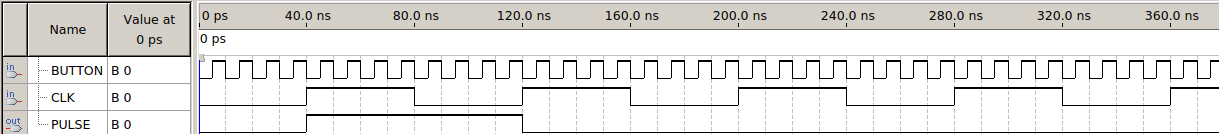
\includegraphics[scale=0.5]{debounderresults}
	\end{center}
\end{figure}

\chapter*{Testing the \texttt{g07\_stack} Circuit}
\addcontentsline{toc}{chapter}{Testing the \texttt{g07\_stack} Circuit}
Before testing the testbed on the DE1 board, it was decided to do a thorough test of the
\texttt{g07\_stack} circuit's core functionality on its own. This made drawing test case waveforms
for all of the BJT operations simpler. Sample output waveforms are given below.
\begin{figure}[h]
	\begin{center}
		\caption{Initial operations}
		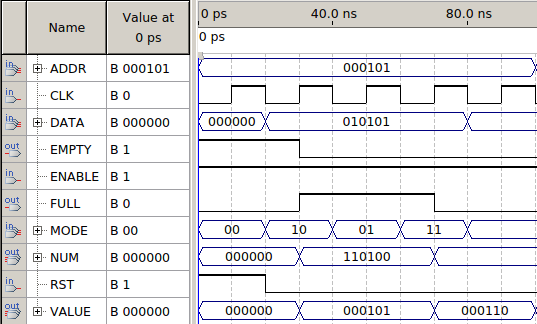
\includegraphics[scale=0.47]{stacktest_1}
	\end{center}
\end{figure}
This sequence shows that the BJT initializes in an empty state, and after calling init (mode = 10),
\texttt{FULL} goes high and \texttt{EMPTY} goes low. Next, a push operation (mode 01) is attempted,
but no data changes because \texttt{FULL} is high. Then, after pop (mode 11) is called,
\texttt{FULL} goes low and the value stored in address 000101 goes from 000101 to 000110, showing
that the element underneath it was shifted upward after the pop, as expected.
\begin{figure}[h]
	\begin{center}
		\caption{Pop inspection}
		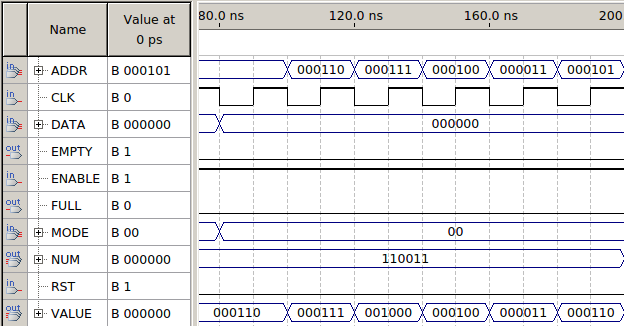
\includegraphics[scale=0.5]{stacktest_2}
	\end{center}
\end{figure}
It can be seen from the next image that after switching the address to 000110, the \texttt{VALUE} is
000111, showing that an element below the pop source received shifted data as well, which is
expected. Then, address 000111 is expected showing again that shifting below the pop source is
functional. Next, address 000100 was observed to be storing 000100, showing that data above the
source of the pop was not affected, which is also expected. This trend was consistent at address
000011 as well. Note that the value of \texttt{NUM} is 110011, representing 51 in decimal, because
one element was popped.\\\\
\begin{figure}[h]
	\begin{center}
		\caption{Push inspection}
		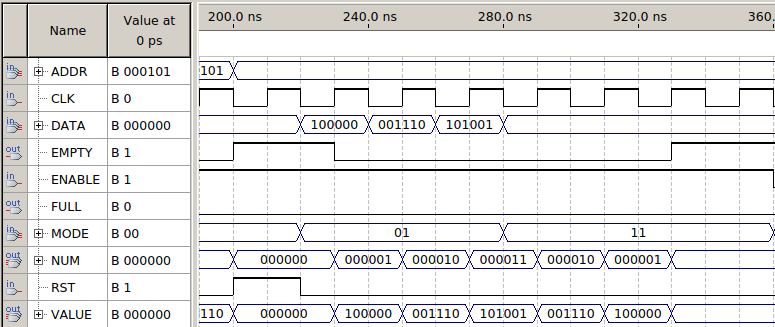
\includegraphics[scale=0.6]{stacktest_3}
	\end{center}
\end{figure}
At this stage, \texttt{RST} was set high for a clock pulse, and consequently \texttt{NUM}, as well
as the data stored in the flip flops, are set to 0. Following the reset, the numbers 100000, 001110,
and 101001 are pushed to the stack, and are observed sequentially at address 0. Furthermore,
\texttt{NUM} increments after each push.\\
\begin{figure}[h]
	\begin{center}
		\caption{Resistence inspection}
		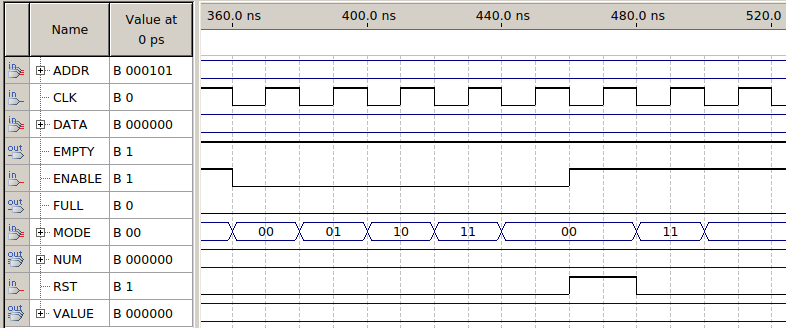
\includegraphics[scale=0.6]{stacktest_4}
	\end{center}
\end{figure}
Then, \texttt{ENABLE} was set low while each operation was attempted. It can be seen that in the
interval where \texttt{ENABLE} is low, no other outputs change, which is expected. Finally,
\texttt{RST} was set high once again, bringing \texttt{NUM} to 0 and \texttt{EMPTY} high. A pop
operation was then attempted (mode 11), but it can be seen that the value of \texttt{NUM} does not
change, and no other outputs change, which is expected.\\\\
The series of tests shown above test all intended functionalities and conditions of the BJT, and all
were shown to be successful.
\chapter*{Testing the Testbed on the Hardware}
\addcontentsline{toc}{chapter}{Testing the Testbed on the Hardware}
Now, the testbed is ready to be tested on the Altera DE1 board. Rather than showing functional
simulations and output waveforms for the testbed (which would be hard because the outputs are 7
segment display codes), a series of photographs was taken to give evidence of the testbed's
functionality.
\begin{figure}[h]
	\begin{center}
		\caption{Initial FPGA configuration}
		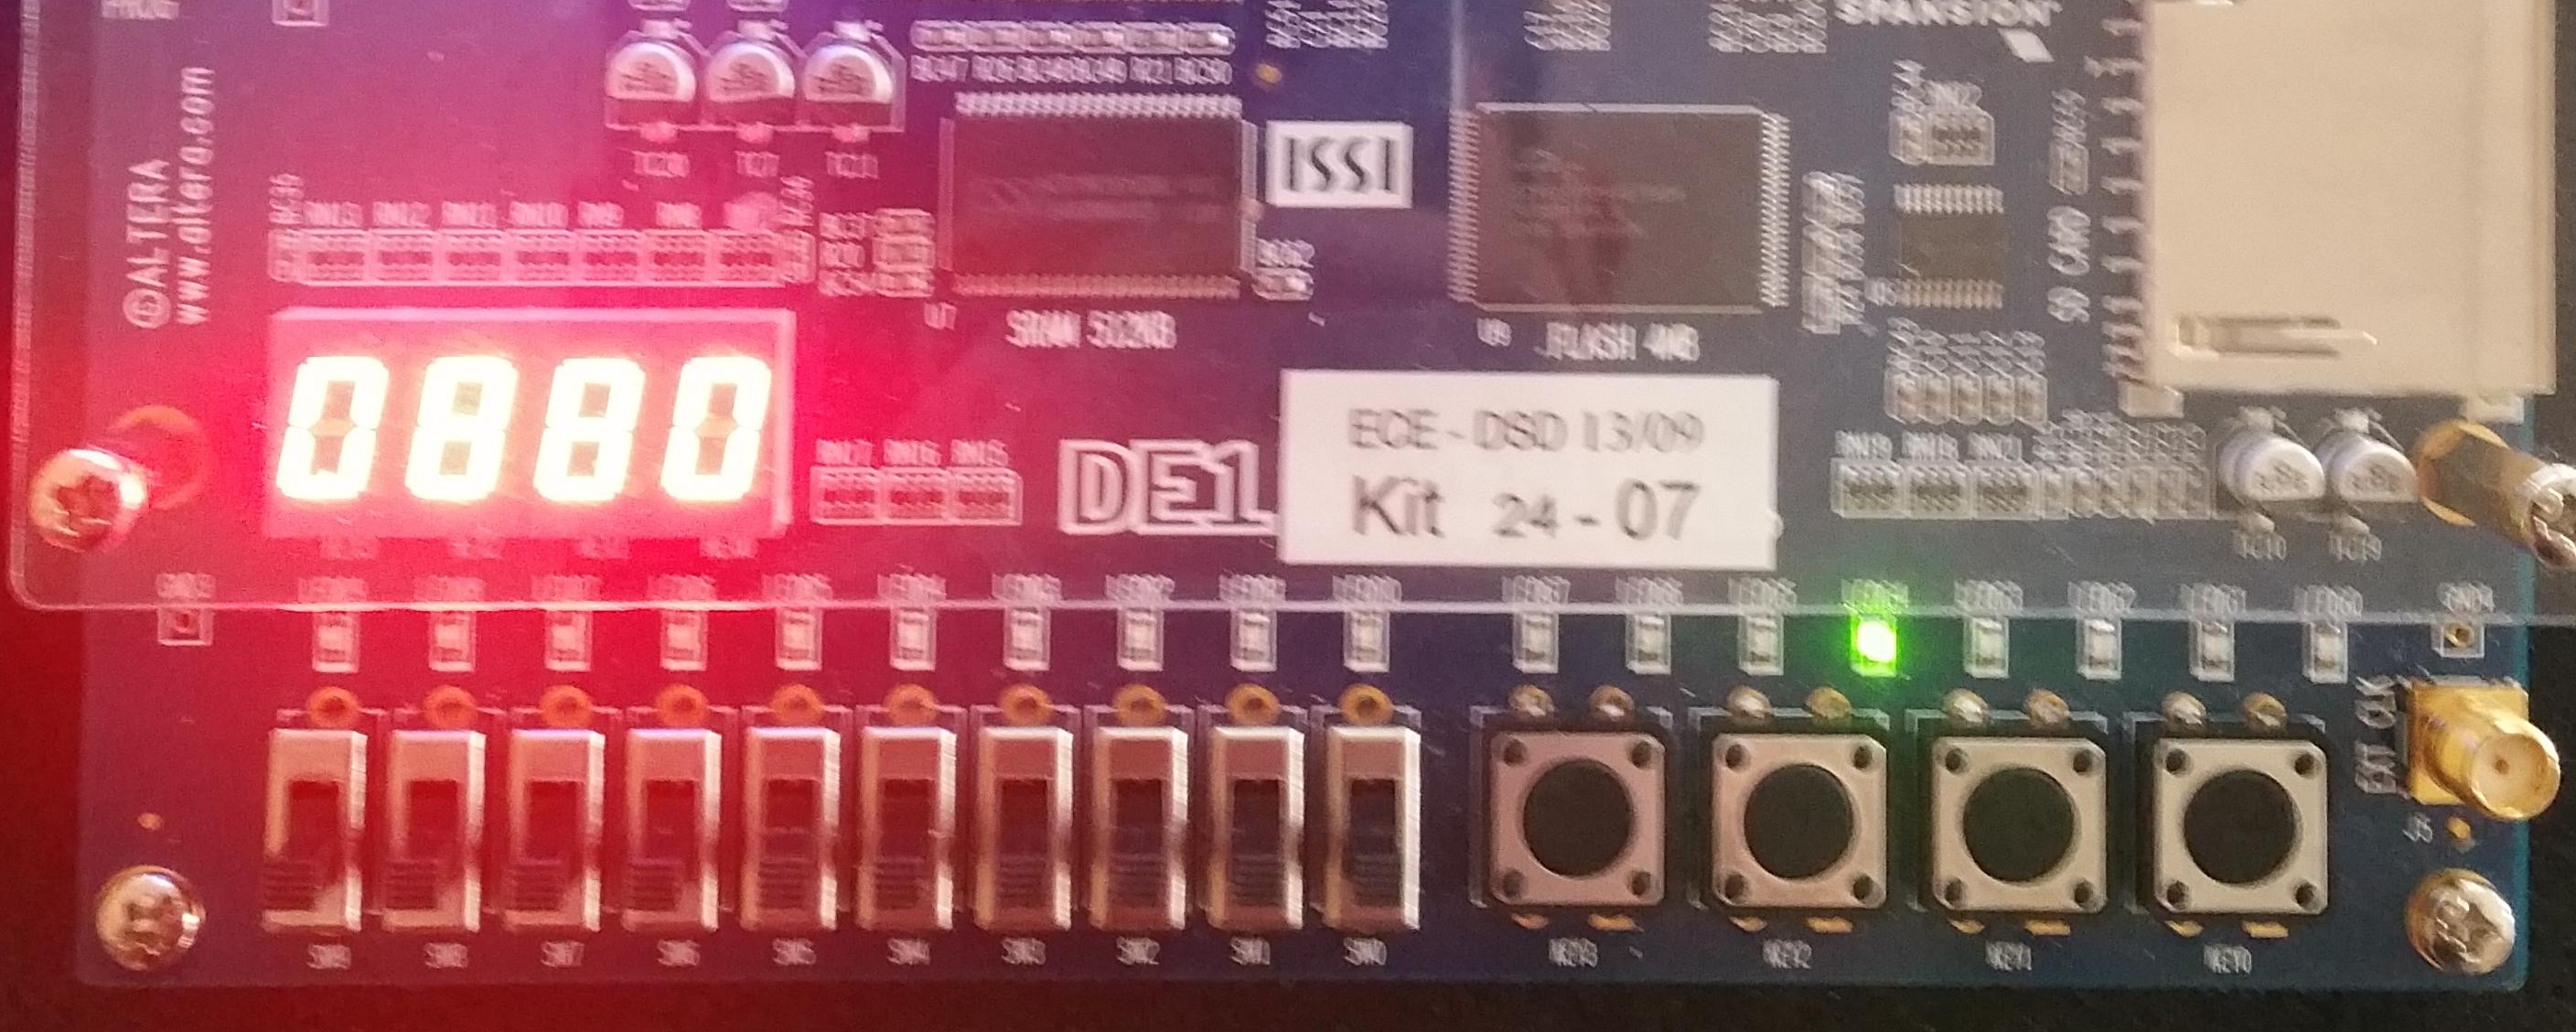
\includegraphics[scale=0.15]{fpga1}
	\end{center}
\end{figure}
Here is how the FPGA board looks when the testbed is first loaded. The buttons, switches, and LED's
of interested are listed below:
\begin{itemize}
	\item The leftmost 7 segment display represents the \texttt{VALUE} output of the stack at a
		given \texttt{ADDR}, modulo 13.
	\item The rightmost 7 segment display represents the floor of the \texttt{VALUE} output at
		\texttt{ADDR} divided by 13.
	\item The six leftmost switches determine the \texttt{ADDR} to get values from in the BJT.
	\item The two rightmost switches determine the \texttt{MODE} input of the BJT.
	\item The leftmost button controls the \texttt{ENABLE} input of the BJT.
	\item The rightmost button controls the \texttt{RST} input of the BJT.
	\item The rightmost LED above the second pushbutton from the left (the LED that is illuminated
		in the first picture) is illuminated when the \texttt{EMPTY} output of the
		\texttt{g07\_stack} is high.
	\item The LED to the left of the \texttt{EMPTY} LED is illuminated when the 
		\texttt{FULL} output of the \texttt{g07\_stack} is high.
\end{itemize}
In the initial configuration, the stack is empty, so surely both 7 segment displays show zero, and
the \texttt{EMPTY} button is illuminated.

\begin{figure}[h]
	\begin{center}
		\caption{Init was carried out}
		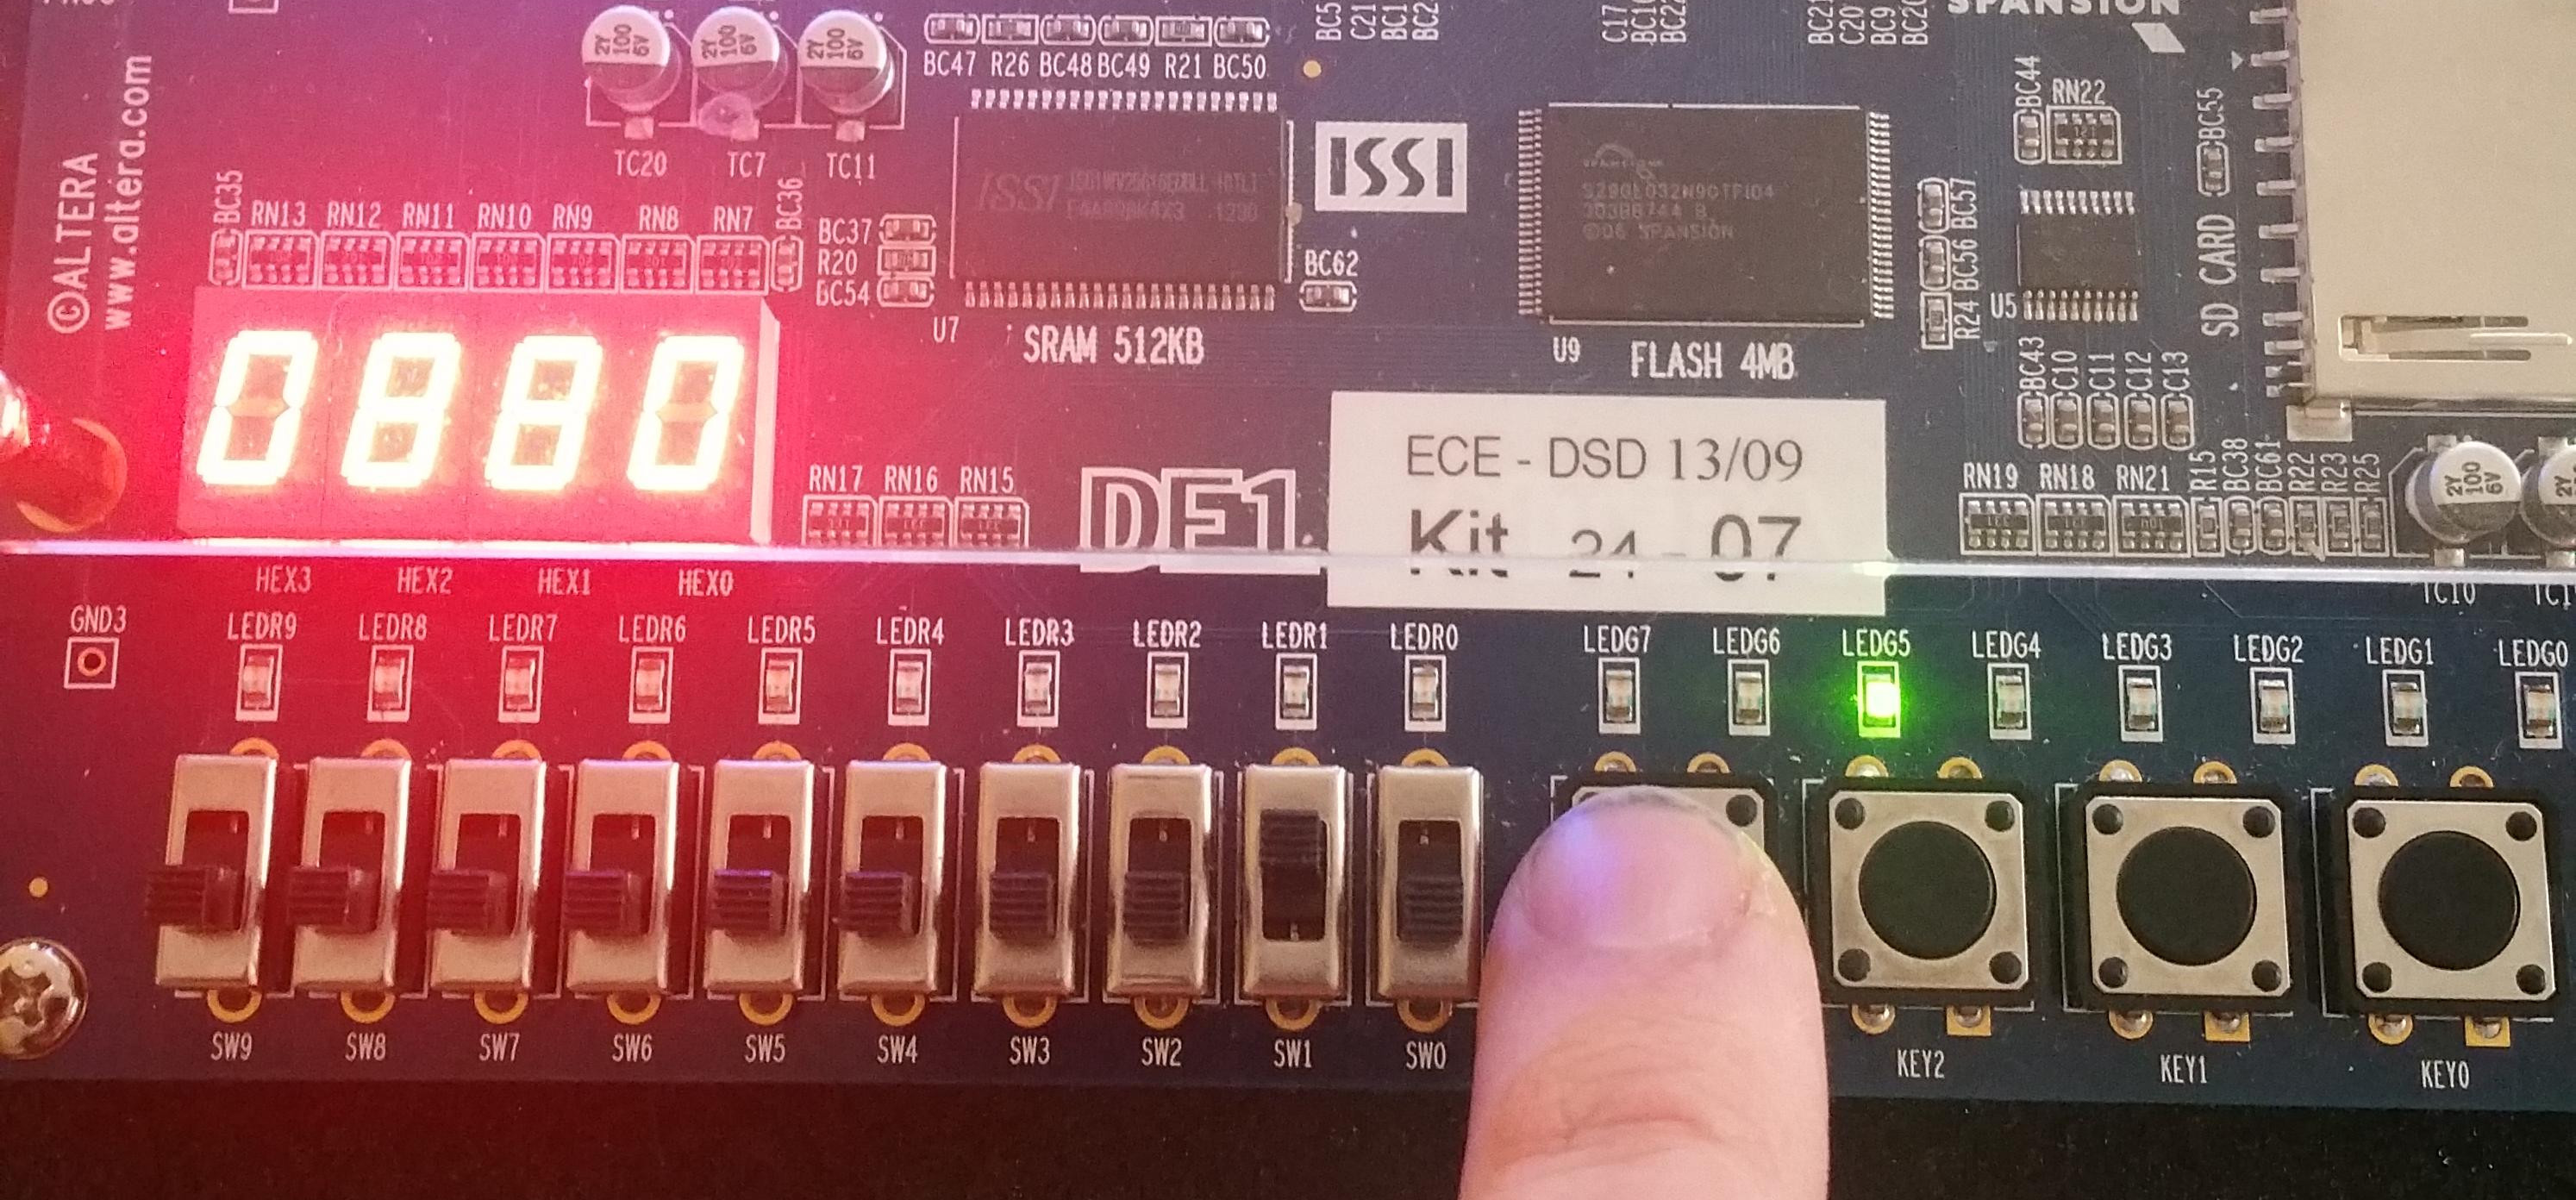
\includegraphics[scale=0.15]{fpga2}
	\end{center}
\end{figure}
Next, the \texttt{MODE} switches were set to 10 to indicate an init operation, and the enable
buttonw was pressed. Since \texttt{ADDR} is still 0, the 7 segment displays show zero, however it is
important to note that the \texttt{EMPTY} LED is now off, and the \texttt{FULL} LED is on.

\begin{figure}[h]
	\begin{center}
		\caption{Changing \texttt{ADDR}}
		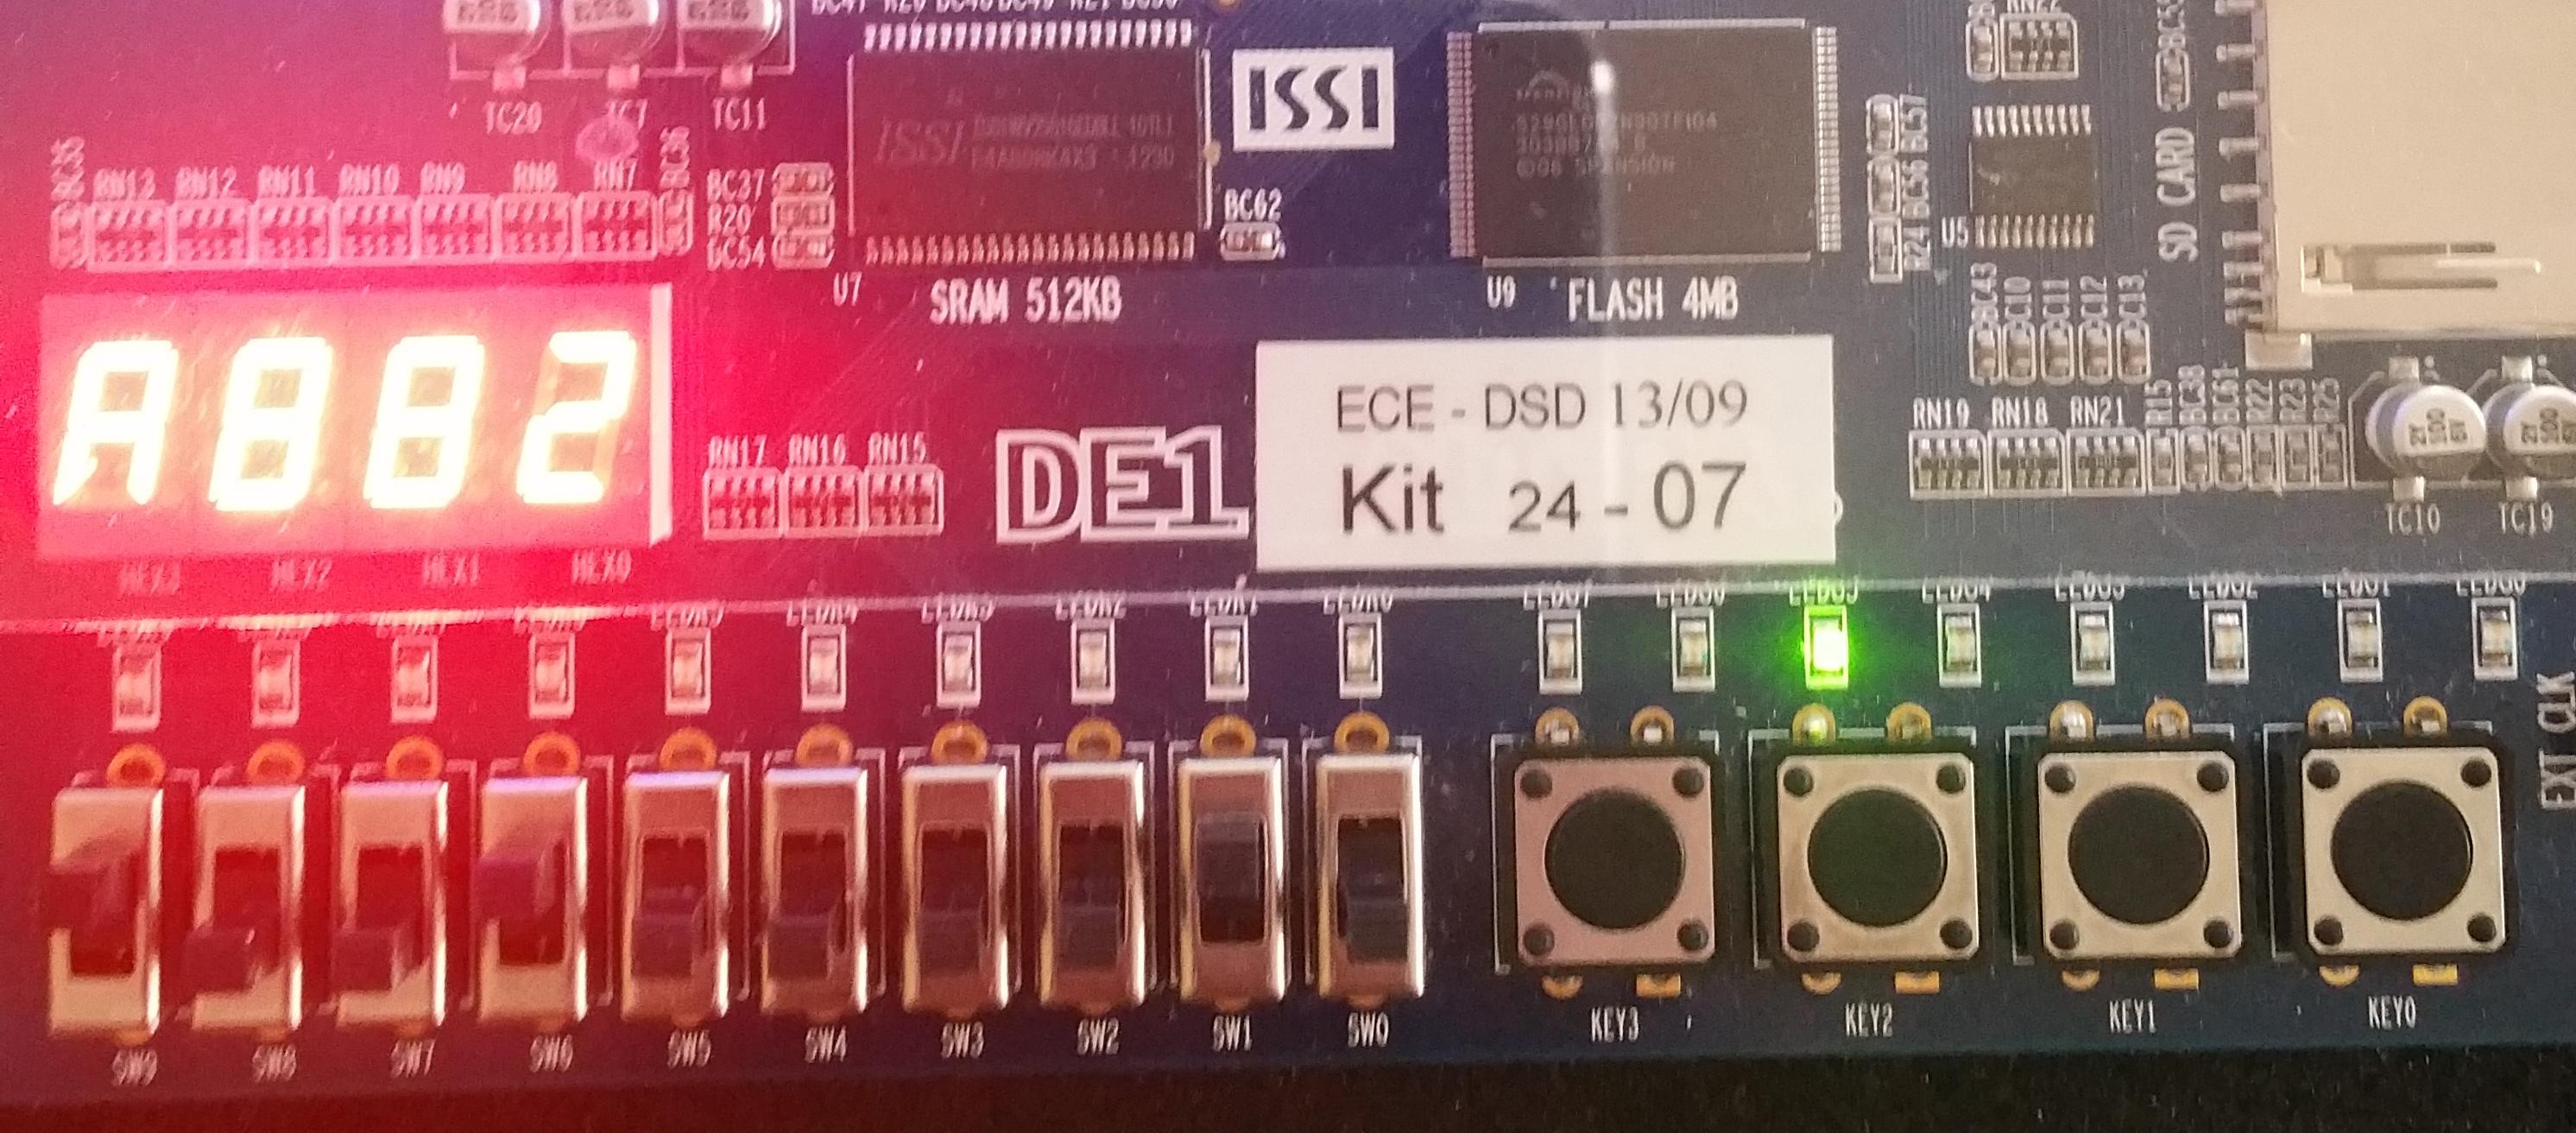
\includegraphics[scale=0.15]{fpga3}
	\end{center}
\end{figure}
At this stage, \texttt{ADDR} was changed to a value of 100100. The 7 segment displays show A2, which
represents $2*13 + A = 26 + 10 = 36_{10} = 100100_2$. Thus, the data is correct.

\begin{figure}[h]
	\begin{center}
		\caption{Trying a pop operation}
		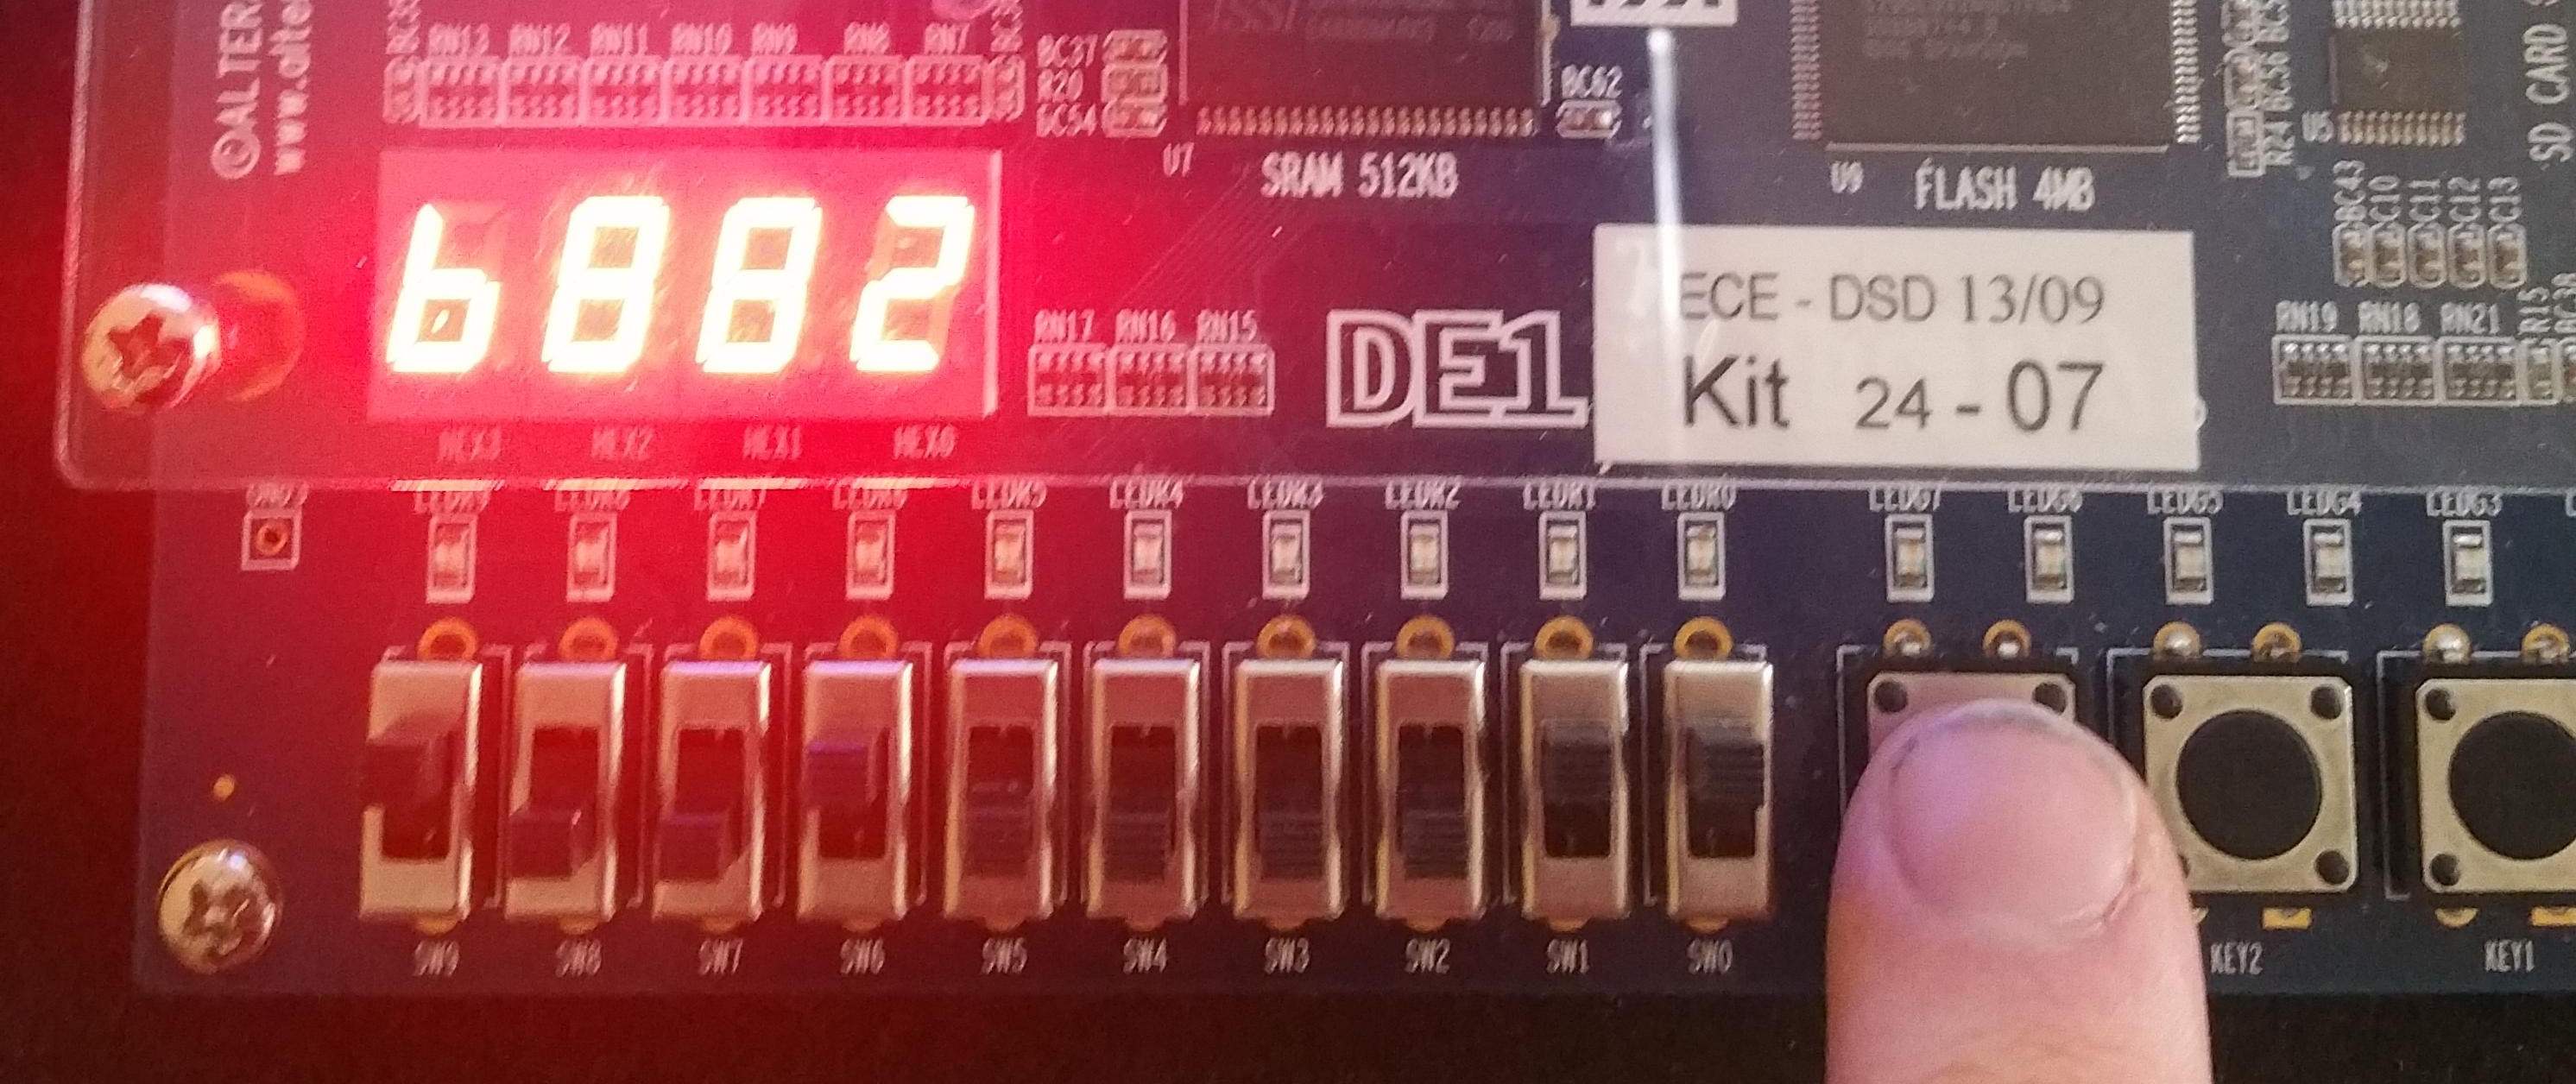
\includegraphics[scale=0.15]{fpga4}
	\end{center}
\end{figure}
Next, the mode buttons were set to 11, indicating a pop operation. The enable button was pushed once
and the 7 segment displays show B2, which is one larger than A2. Therefore, the data from the cell
below 100100 was shifted into 100100, implying that \textit{one} pop operation has taken place. This
confirms the functionality of the \texttt{g07\_debounder}. Furthermore, it is clear now that both
\texttt{EMPTY} and \texttt{FULL} LED's are off, because now the stack is neither full or empty.

\begin{figure}[h]
	\begin{center}
		\caption{Trying another pop operation}
		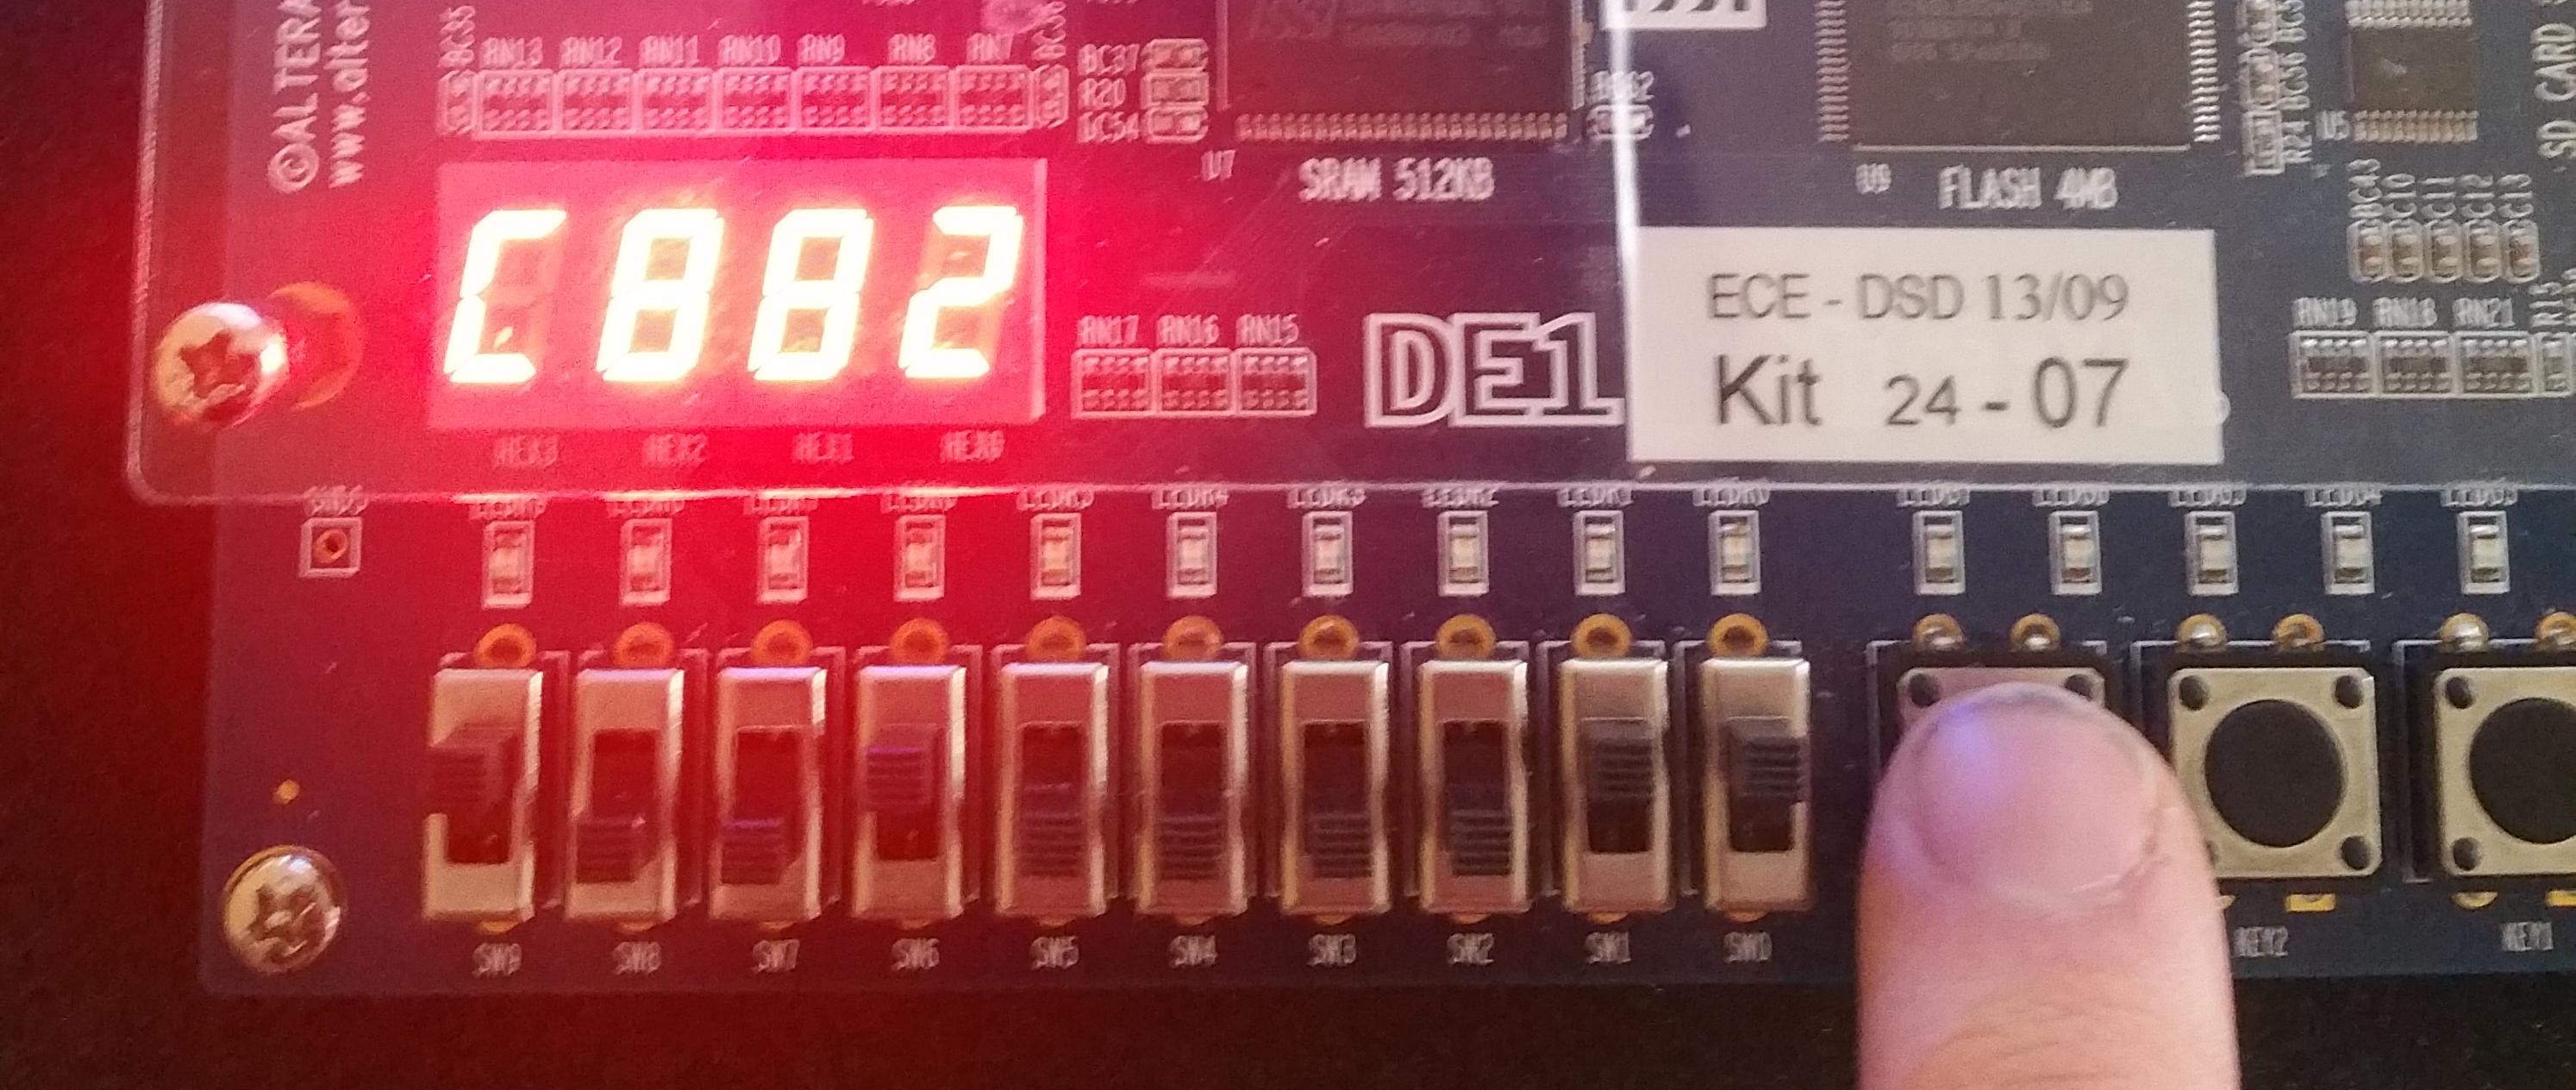
\includegraphics[scale=0.15]{fpga5}
	\end{center}
\end{figure}
Then, the enable button was pushed again, allowing for another pop operation. This time, the 7
segment display shows C2, which is one greater than B2, so another pop operation was shown to be
successful.

\begin{figure}[h]
	\begin{center}
		\caption{Trying a pop operation}
		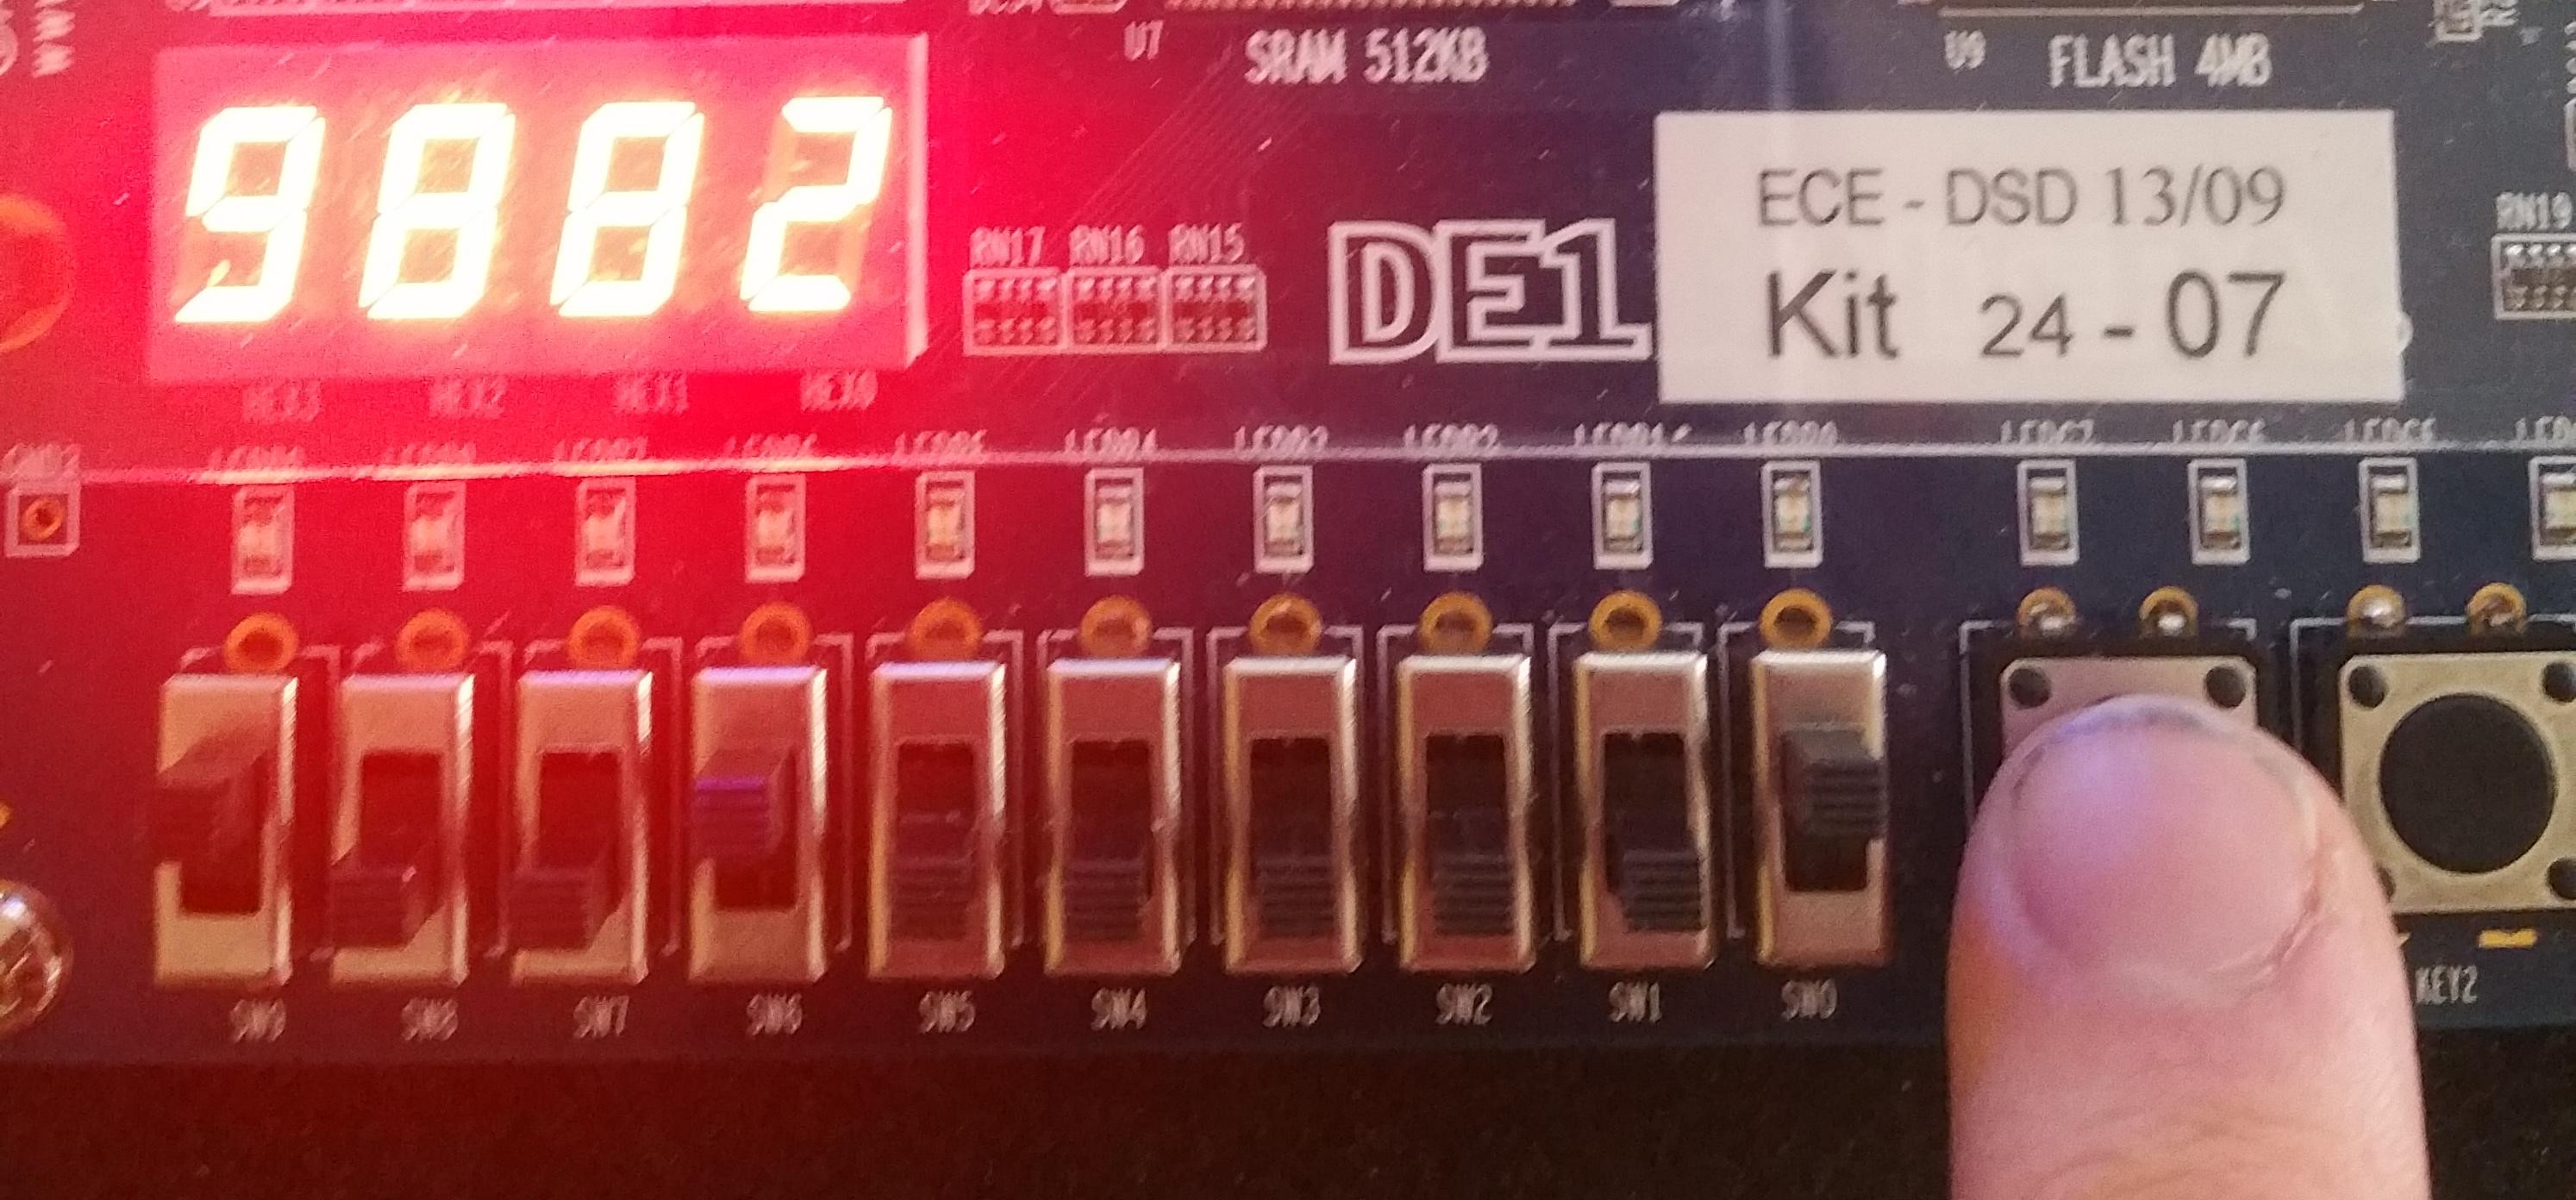
\includegraphics[scale=0.15]{fpga6}
	\end{center}
\end{figure}
Finally, the mode buttons were set to 01, indicating a push operation, and the enable button was
pressed. The 7 segment displays show 92. Since the values A2 and B2 were popped off the stack, the
next value on the BJT above the current address must be 92 (one less than A2), which shows that
the BJT's push and pop are operating properly, and once again shows that the \texttt{g07\_debounder}
is working. \\\\
It is important to note that the purpose of these tests on the DE1 board was not to test the
functionality of the BJT implementation itself, but rather the testbed. It was already shown that
the \texttt{g07\_stack} is functional, so all that was left to be shown was the functionality of the
\texttt{g07\_debounder}, the proper codes being sent to the 7 segment displays, and the proper pin
assignments to the DE1. All of these functionalities were shown to be successful in these tests.

\part{The Results}
\chapter*{The Plight of the \texttt{g07\_stack} and its Companions}
\addcontentsline{toc}{chapter}{The Plight of the \texttt{g07\_stack} and its Companions}
The following data were taken from Quartus II's divine analysis of the testbed circuit. Note that
the testbed circuit contains a \texttt{g07\_stack} as well as the 7 segment decoders, the
\texttt{mod13} circuit, and the almighty \texttt{g07\_debounder}.
\section*{The Flow Summary}
\addcontentsline{toc}{section}{The Flow Summary}
\begin{figure}[h]
	\begin{center}
		\caption{Tabulated results from Quartus II's Flow Summary}
		\begin{tabular}{|c|c|}
			\hline
			\textbf{Total Logic Elements} & 4\%\\\hline
			Total Combinational Functions & 4\%\\\hline
			Dedicated Logic Registers & 2\%\\\hline
			Total Registers & 344\\\hline
			Total Pins & 9\%\\\hline
			Total Virtual Pins & 0\\\hline
			Total Memory Bits & 1\%\\\hline
			Embedded Multiplier 9-bit Elements & 0\\\hline
			Total PLL's & 0\\\hline
		\end{tabular}
	\end{center}
\end{figure}

The table above shows statistics regarding how much of the Cyclone II's hardware is being used by
the testbed. These results are more-than-reasonable considering the magnitude of the circuit being
implemented.
\section*{The Timing Analysis}
\addcontentsline{toc}{section}{The Timing Analysis}
To determine the feasibility of the testbed with regard to speed, Quartus II's TimeQuest Timing
Analyzer was used. This tool was used to calculate the longest path of data within the testbed, and
reported that this path required a maximum clock frequency of 158.93 MHz. Given the 50 MHz clock
frequency maximum on the DE1 board, this restriction is not very restricting, and is perfectly
acceptable.
\begin{appendices}
	\chapter{Haskell Code for \texttt{g07\_generator}}
	\label{app:hs}
	\lstinputlisting[language=Haskell]{Lab3/generator.hs}
	\chapter{VHDL Code tor \texttt{g07\_testbed}}
	\label{app:testbedvhdl}
	\lstinputlisting[language=Java]{Lab3/g07_testbed.vhd}
	\chapter{Schematic of the \texttt{g07\_debounder}}
	\label{app:debounder}
	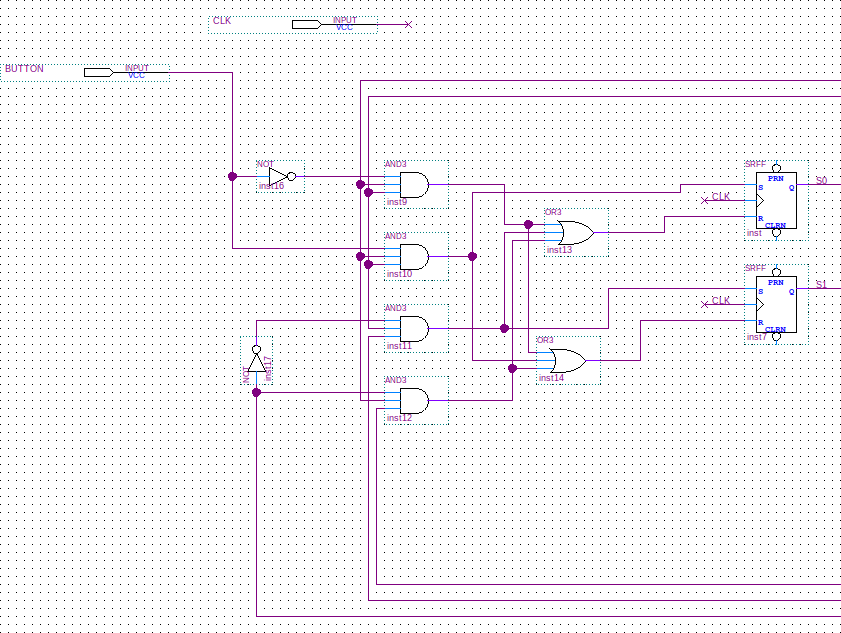
\includegraphics[scale=0.4,angle=0]{debounder1}\\
	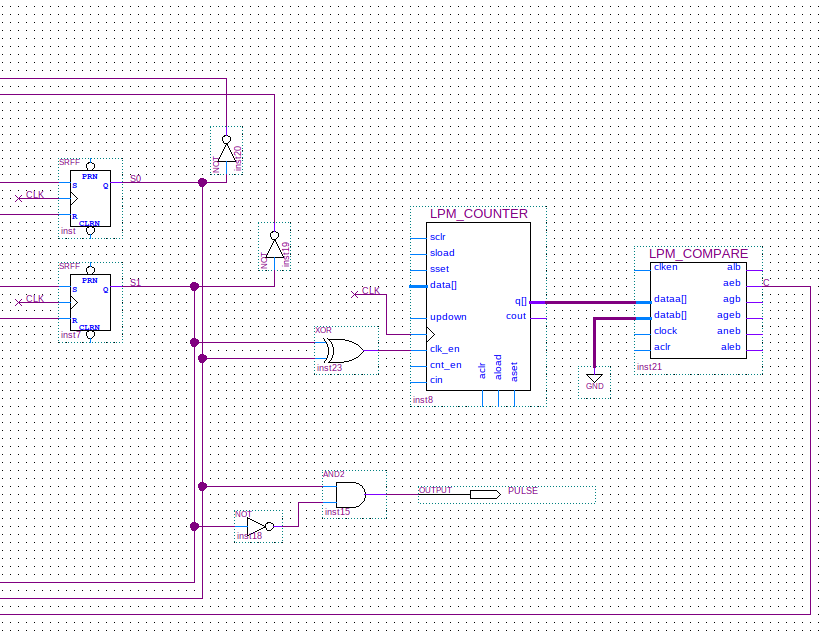
\includegraphics[scale=0.37,angle=0]{debounder2}
\end{appendices}
\bibliographystyle{ieeetr}
\bibliography{sources}
\end{document}
